\begin{figure}[H]
    \centering

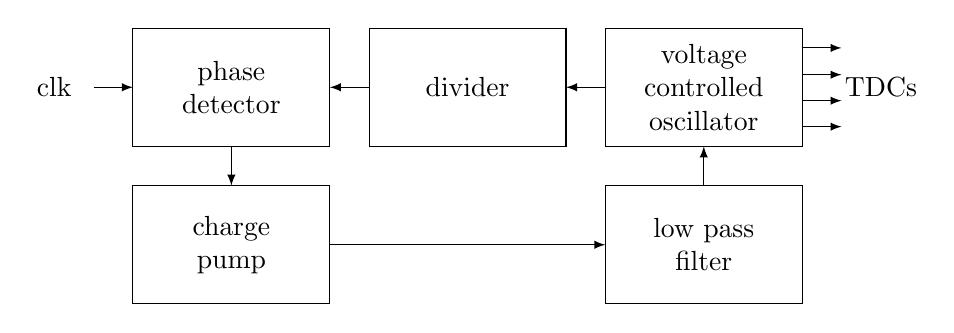
\begin{tikzpicture}

\draw  (-2,1.75) rectangle (0.5,0.25) node[pos=.5, align=center]{phase\\detector};
\draw  (1,1.75) rectangle (3.5,0.25) node[pos=.5, align=center]{divider};
\draw  (4,1.75) rectangle (6.5,0.25) node[pos=.5, align=center]{voltage\\controlled\\oscillator};
\draw  (4,-0.25) rectangle (6.5,-1.75) node[pos=.5, align=center]{low pass\\filter};
\draw  (-2,-0.25) rectangle (0.5,-1.75) node[pos=.5, align=center]{charge \\pump};

\draw [>=latex, ->] (1,1) -- (0.5,1);
\draw [>=latex, ->] (4,1) -- (3.5,1);
\draw [>=latex, ->] (0.5,-1) -- (4,-1);
\draw [>=latex, ->] (-0.75,0.25) -- (-0.75,-0.25);
\draw [>=latex, ->] (5.25,-0.25) -- (5.25,0.25);
\draw [>=latex, ->] (-2.5,1) -- (-2,1);

\draw [>=latex, ->] (6.5,1.5) -- (7,1.5);
\draw [>=latex, ->] (6.5,1.16) -- (7,1.16);
\draw [>=latex, ->] (6.5,.83) -- (7,.83);
\draw [>=latex, ->] (6.5,0.5) -- (7,0.5);


\node at (-3,1) {clk};
\node at (7.5,1) {TDCs};
\end{tikzpicture}
    \caption{schematic of phase locked loop generating signals for TDCs}
    \label{tkz:PPL}
\end{figure}